Creative AI, such as using deep learning models to generate paintings and music, has been a popular research domain. Since creative activities are representative of unique human intelligence, numerous works have attempted to replicate the creative process on machines.
For example, Pharmako-AI \citep{allado-mcdowell_okojie_2020} is a book co-written by K Allado-McDowell and GPT-3 \citep{gpt3} through exchanges between the human and the language model. 
Works like DALL-E, GLIDE, and DALL-E 2 tackle the problem of synthesizing images from short language descriptions, and these generative models have produced many imaginative and inspring art pieces \citep{dallePaper,glidePaper,dalle2Paper}.
These work are often motivated by the vision to create machines that can interact with people and augment human creativity.  
Our work is driven by a similar vision: how can we build systems that can be creative like humans so that AI agents and people can pariticpate in creative activities together and inspire each other. 

\begin{figure*}[!htb]
\centering
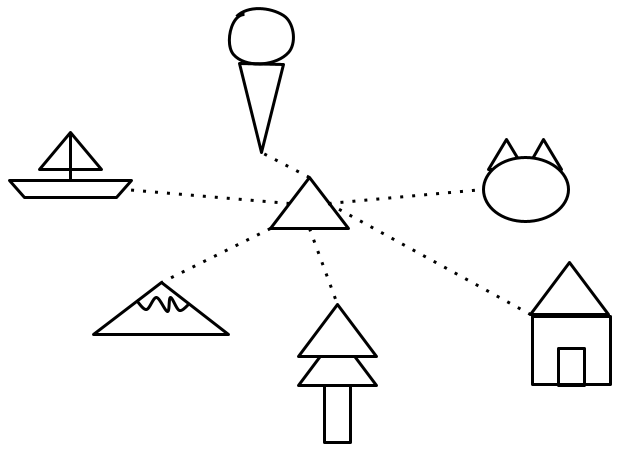
\includegraphics[width=.3\linewidth]{introduction/sketch_composition.png}  
\caption{.}
\label{introduction.composition}
\end{figure*}

Instead of studying how to generate realistic art works from a wide range of domains like DALL-E, we approach creativity from a different angle and investigate composition of basic visual concepts to create different object sketches. 
An example is illustrated in Figure \ref{introduction.composition}: a triangle can be a boat sail, a ice-cream cone, a cat ear, a house roof, a tree canopy, a mountain, etc. The same triangle is morphed to become different parts in sketches of different objects. 
In a similar way, words in language are also applied in different contexts, and their meanings shift depending on the usage. For example, the word \textit{large} in \textit{a large scoop of ice-cream} and \textit{a large cat face} implies size at different scales and conjure up different imagery. The large scoop of ice-cream is probably oveflowing from the little cone underneath with the melting ice-cream dripping from the side, while the large cat face implies a chubby round face compared to the cute pointy ears at the top. 

Can we build systems that can compose basic parts in a similar manner and transfer their descriptions 
In this thesis, we look at semantic parts in sketches (for example, a sketch of ice-cream contains two semantic parts: a scoop of ice-cream and a cone) and how people describe 

% [B]
They might not look exactly like their natural image correspondence. 
Sketches abstract away the details in natural images but do not fall short in illustrating properties of the objects. Its abstractness allows for more creativity.
Human can compose simple geometric shapes to create figures that represent a wide variety of objects and concepts in the world. Icons and emojis are in this category: the amount of information these symbols convey contrasts with the simplicity of the figures. 

% [B]
Sketches illustrate the core features. We are skilled at abstracting away the details but capture the most essence of the object to make them distinguishable.

% [B] 
The ability to still get the idea across with such simple toolkit proves human creativity. We don't need complicated detailed realistic sketches, a few simple strokes are able to convey what we want to say. This type of creativity is innate. It is a creativity that we are born with: we start doodling as kids. We start scribbling on walls before knowing that we are re-creating our experience onto a canvas. It is the sort of creativity that lies on every one of us, and there is no high bar or artistic requirement to express this kind of creativity.

% [B]
Language creates space for imagination. Language creates room for creativity. The ambiguity in language. Large face. How large. Curved wings abstract away the details of the wings.

% [B]
Language transfer